\documentclass[12pt]{article}

%---------------------------------------------------------------------------
% Packages, Encoding, Margins, Euro sign
\usepackage[english]{babel}
\usepackage[T1]{fontenc}
\usepackage[latin1]{inputenc}
%\usepackage[utf8]{inputenc}
\usepackage{url}
\usepackage{eurosym}
\usepackage{fullpage}

\usepackage{listings}
\usepackage{color}
\definecolor{BrightGrey}{rgb}{0.98,0.98,0.98}
\definecolor{Red}{rgb}{1.0,0.0,0.0}
\definecolor{Green}{rgb}{0.0,0.3,0.0}
\definecolor{Blue}{rgb}{0.0,0.0,0.3}

\lstdefinestyle{Bash}
               {language=Bash,
backgroundcolor=\color{BrightGrey},
commentstyle=\color{Green},
stringstyle=\color{Blue},
showstringspaces=false,
basicstyle=\small\color{black},
numbers=none,
captionpos=b,
tabsize=4,
breaklines=true
}

\lstdefinestyle{Python}
               {language=Python,
backgroundcolor=\color{BrightGrey},
commentstyle=\color{Green},
stringstyle=\color{Blue},
showstringspaces=false,
basicstyle=\small\color{black},
numbers=none,
captionpos=b,
tabsize=4,
breaklines=true
}

\lstdefinestyle{C++}
               {language=C++,
backgroundcolor=\color{BrightGrey},
commentstyle=\color{Green},
stringstyle=\color{Blue},
showstringspaces=false,
basicstyle=\small\color{black},
numbers=none,
captionpos=b,
tabsize=4,
breaklines=true
}

%---------------------------------------------------------------------------
% Font packages
\usepackage{charter}

%---------------------------------------------------------------------------
% If tables are being used...
\usepackage[table]{xcolor}

\usepackage{graphicx}
\usepackage{amsmath}

%---------------------------------------------------------------------------
\begin{document}

%---------------------------------------------------------------------------
% Document title, author, date, ...
\title{libga (MPI)}
%\author{Martin Wirth}
\date{V 2013.1}
\maketitle
\thispagestyle{empty}

\tableofcontents

%---------------------------------------------------------------------------
% Content

\section{Motivation}
The libga (MPI) library is actually a set of tools that allow its user to solve optimization problems using genetic algorithm (GA) techniques. Both C++ and Python (>= 2.7) libraries are provided. Only a very limited set of algorithms are supported: for multi-objective problems a variation of the Strength Pareto Evolutionary Algorithm (SPEA2) \cite{Zitzler01spea2:improving} has been implemented. The single-objective variant (SGA) does not follow a specific algorithm but it includes the typical steps of a GA, namely evaluation, selection, crossover and mutation. SGAs usually employ an elitism scheme which is also available in libga. \\
The idea behind this implementation is to offer a relatively simple to use set of tools and not a comprehensive scientific survey of operators and algorithms found in other libraries. \\
Both the single- and the multi-objective variants (C++ and Python libraries) can be run in a single-threaded environment or as MPI processes. The example scripts and test applications are written for use with MPI. The interfaces of the single-threaded and the MPI versions are almost identical so very little change is needed to go parallel. \\
The C++ versions expect to deal with real-valued optimization problems only. This is simplifying the GA's implementation and also the communication over MPI. The Python versions are generic enough that the genome type is not important as long as it is array-like. The elements of the genome (i.e. the solution candidates) could be arrays, trees or anything else. However, libga only offers crossover operators for the typical real-valued case. You would have to supply your own custom operators for other genome types. Your custom solution type would have to be able to be ``pickled'' to be sent via MPI aswell. This is dependent on mpi4py's behavior. 

\section{Obtaining the Source}
Right now the source is distributed as a tar.gz file named ``libga\_mpi.tar.gz''. Extract it into a directory. 

\section{Prerequisites}
\begin{enumerate}
  \item Working C++ toolset supporting C++11 (tested with Clang 3.3)
  \item CMake (Version >= 2.6)
  \item Python (Version >= 2.7)
  \item MPICH2 
  \item mpi4py
  \item NumPy
  \item SciPy
  \item Matplotlib
\end{enumerate}

\section{Compiling and Running Examples}
The ``examples'' directory in the source distribution includes a number of shell scripts that both build and run a few test problems. 

%---------------------------------------------------------------------------
% Table example
\begin{table}[ht]
\caption{Example scripts}
\begin{center}
\rowcolors{1}{BrightGrey}{white}
\begin{tabular}{  l | p{10cm}  }
  \hline
   File name & Description \\
  \hline
  native\_build\_and\_run\_kursawe & Builds all C++ test applications in the ``build'' directory then runs them in an MPI context. The results of each process are merged and displayed in a Matplotlib graph. You can click data points to display more information in the terminal. \\
  native\_build\_and\_run\_rastrigin & Builds all C++ test applications in the ``build'' directory. It runs the rastrigin problem in an MPI context. Results are merged and the fittest (i.e. best fitting) solution is displayed in the terminal. For the rastrigin problem the fitness should be close to zero. The variables themselves are also approaching zero for a global minimum.  \\
native\_build\_and\_run\_MOP5 & Same as the above but runs the MOP5 (Viennet) problem. Displays the three-dimensional objective space using Matplotlib. \\
  python\_run\_kursawe & Run the kursawe test problem (Python implementation) in an MPI context. Merges results and displays them in a Matplotlib graph. \\
  python\_run\_rastrigin & Run the rastrigin test problem (Python implementation) in an MPI context. Merges results and prints the fittest solution candidate to the terminal \\
python\_run\_MOP5 & Run the MOP5 (Viennet) problem and displays the three-dimensional objective space. \\
  \hline
\end{tabular}
\end{center}
\end{table}
If you do not want to run everything at once execute this in the source directory:
\begin{lstlisting}[style=Bash]
$  mkdir build && cd build
$  cmake .. && make
\end{lstlisting}
This produces three executables ``kursawe'', ``mop5'' and ``rastrigin''. 
\section{Example}
We try to find optimal values for the Kursawe\cite{Kur91} test problem: minimize both \begin{math}
f_{1}(x)\end{math} and \begin{math}f_{2}(x)\end{math} where
\begin{align}
f_{1}(x) &= \sum_{i=1}^{n-1} \left[ -10 \; exp  \left( -0.2 \sqrt{ x_{i}^{2} + x_{i+1}^{2} }  \right) \right] \\
f_{2}(x) &= \sum_{i=1}^{n} \left[ |x_{i}|^{0.8} + 5 \; sin\left(x_{i}^{3} \right) \right] 
\end{align}
\begin{math}n\end{math} is the length of the solution vector (typically 5) and \begin{math}x \in \left[-5,+5\right]\end{math}. \\
To execute the kursawe test problem in an mpi context use
\begin{lstlisting}[style=Bash]
$  mpiexec -n 8 ./kursawe
\end{lstlisting}
This will write eight files called ``kursawe\_data\_0'', ...,''kursawe\_data\_7''. Each process has written its own set of results. A couple of Python scripts are provided which can be used to post-process the results, effectively merging them and recalculating fitness information. 
\begin{lstlisting}[style=Bash]
$  python ../py/merge_to_npz.py ``kursawe_data_*'' 2 test.npz
\end{lstlisting}
This combines all information in the numpy binary file ``test.npz''. \\
Note that ``kursawe\_data\_*'' is a wildcard expression. Any valid bash expression for filtering file names is accepted here. The argument ``2'' tells the merge script that the objective space of the kursawe test problem is two-dimensional. When in doubt, the scripts all display a short example usage string when invoked with the wrong (or zero) number of arguments. \\
You can then proceed and display all of this data using Matplotlib: 
\begin{lstlisting}[style=Bash]
$  python ../py/paretoplot.py test.npz
\end{lstlisting}
This produces a graph very similar to this image: \\
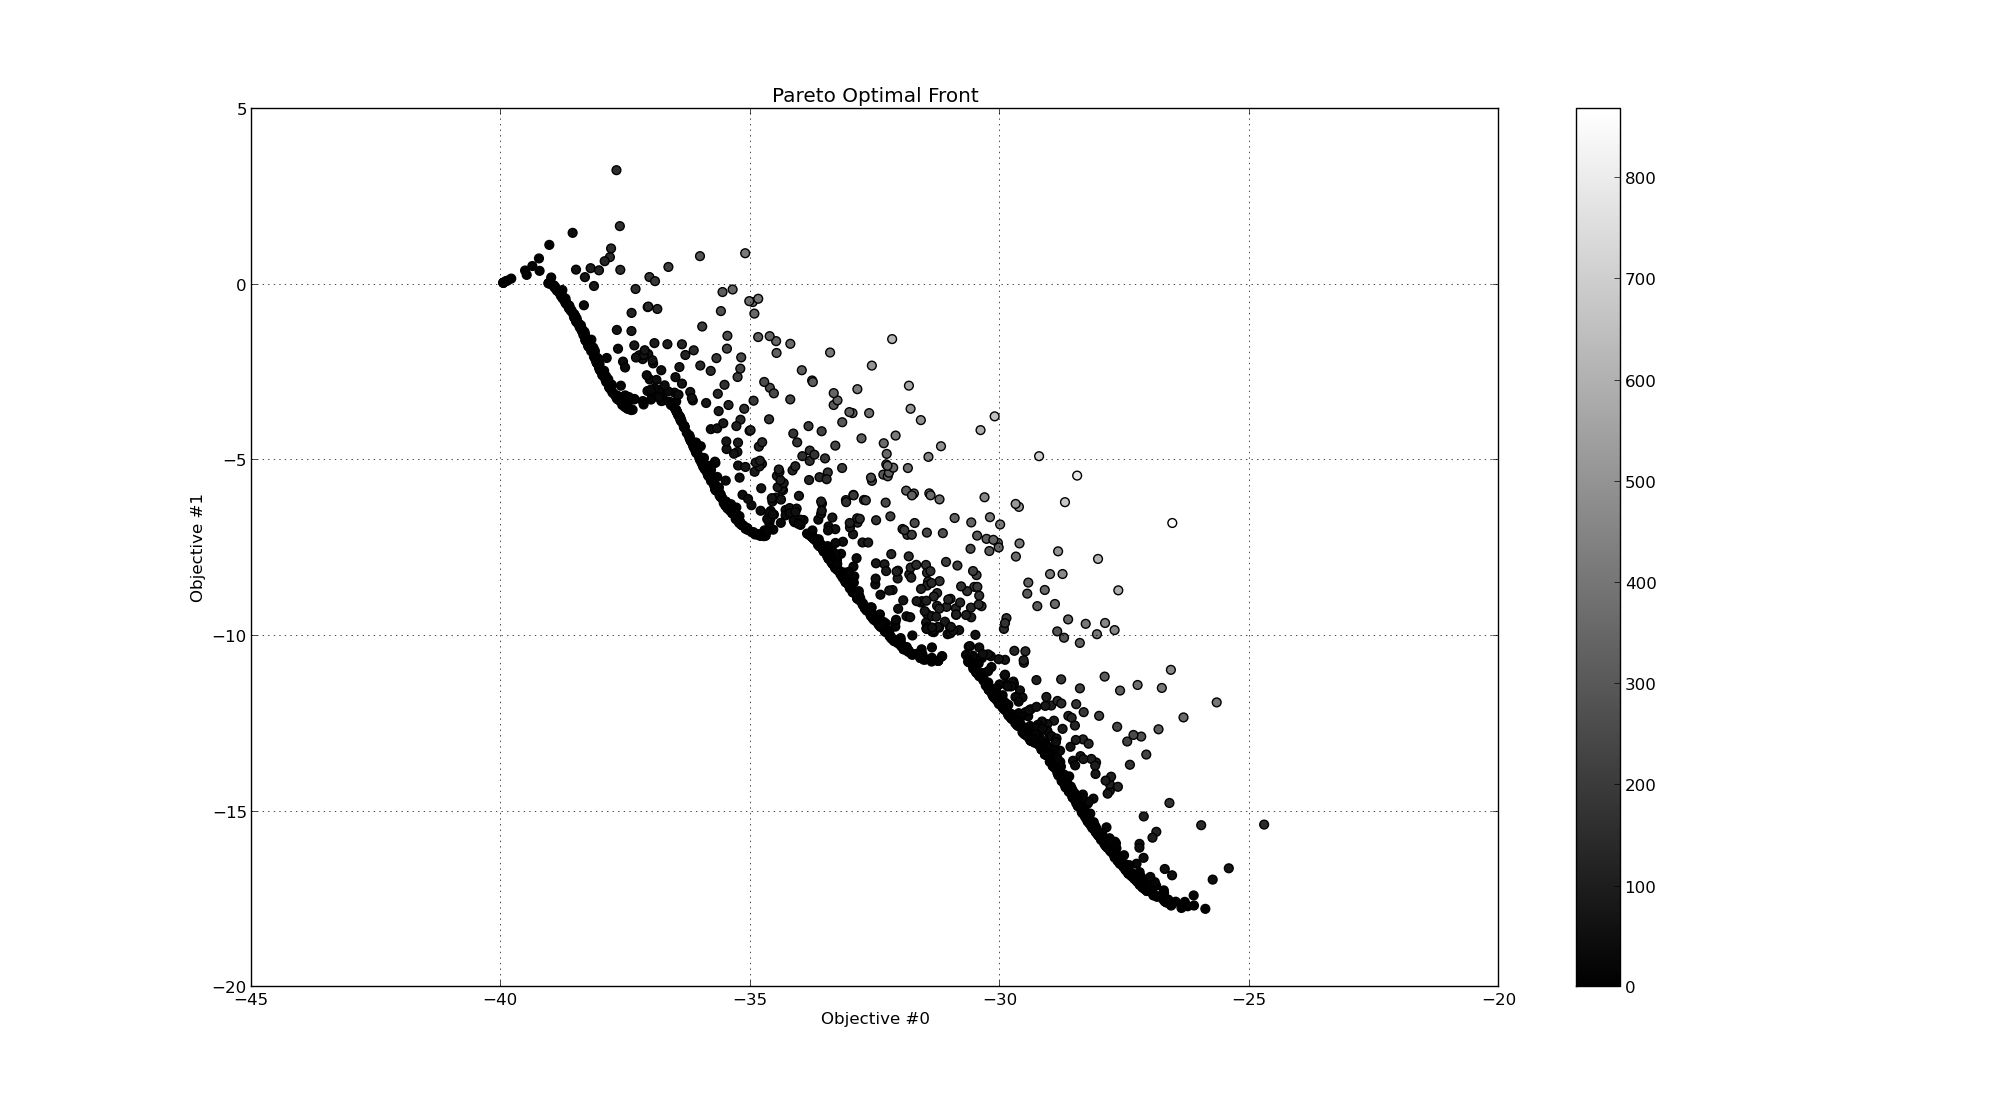
\includegraphics[scale=.4]{example.png} \\
You can click each data point and view the solution's variables, objective values and fitness in the terminal. If too many data points are displayed and you want to reduce the amount of points to just the pareto optimal front you can pre-filter the plot's input data: 
\begin{lstlisting}[style=Bash]
$  python ../py/merge_to_npz.py ``kursawe_data_*'' 2 test.npz
$  python ../py/filter.py test.npz test.npz
$  python ../py/paretoplot.py test.npz
\end{lstlisting}

\section{Python library notes}
libga is designed in a way that supports a certain workflow for working on new optimization problems. If you are tackling a new problem oftentimes writing it down in Python is a good way to start exploring things. In the following section you will find a guide for the most important steps for running the opzimizaion algorithm in Python. We will use the Kursawe test function again. 
\subsection{Setting up configuration and environment}
First, you have to define a few settings for running the optimization algorithm: 
\begin{lstlisting}[style=Python]
population  = 100    # number of solution candidates 
                     # (including archive)
variables   = 5      # variables per solution
generations = 200    # algorithm should terminate after n generations
\end{lstlisting}
We define a lambda function that can be used to evaluate our objectives. Because both the SGA and the SPEA2 algorithms are very generic, they only work with lists i.e. the genome data (the set of all candidate solutions) is just a list of lists. In our case - the Kursawe test problem - we want a list of floating-point vectors. None the less we can convert this list of vectors into a numpy matrix. See ''test\_problems.py'' for an example implementation of the Kursawe problem.  
\begin{lstlisting}[style=Python]
kursawe_fn = lambda g: test_problems.test_kursawe(np.asarray(g))
\end{lstlisting}
Both SGA and SPEA2, at least their Python versions, need an initial genome. We generate a random start: 
\begin{lstlisting}[style=Python]
genome = constraints[:,0]+(constraints[:,1]-constraints[:,0])
       * np.random.random(variables) for i in range(population)]
# assert len(genome) == population
\end{lstlisting}
Note, that we cannot create a Numpy matrix here, since SPEA2 and SGA both need a list. We do not want to make a lot of assumptions about the genome to keep the algorithm as generic as possible. This also allows for different kinds of genome types like, for instance, sets of trees. \\
We pass this genome data to an Spea2 instance: 
\begin{lstlisting}[style=Python]
alg = spea2.Spea2(genome)
\end{lstlisting}
You could now run this algorithm instance by calling alg.start(). This executes in a single-threaded context and might be the ideal way to get started for testing purposes. Since libga is built in two layers we can extend the capabilities of our test application by composition. 
\subsection{Wrapping the algorithm for use with MPI}
\begin{lstlisting}[style=Python]
im = island_model.IslandModel(alg)
\end{lstlisting}
This wraps our Spea2 instance in an IslandModel instance which knows how to communicate over MPI and handles migration of solution candidates from one node to the next. The interface of the most important function ``start()'' is the same for both Spea2 and the IslandModel class which makes going from single-threaded to parallel very easy. 
\subsection{Running the opzimization process}
\begin{lstlisting}[style=Python]
success = im.start(
    kursawe_fn   # objective function
      # run until we have reached our prefedined maximum of generations
    , lambda : alg.generation < generations  
      # crossover method (see gacommon.py for implementation)
    , gacommon.blxa_crossover
      # check whether a solution candidate is valid for our purposes
      # this can also unclude more sophisticated tests, not just
      # range checking. 
    , lambda s: gacommon.is_within_constraints(s, constraints)
      # mutation operator
    , lambda s: gacommon.mutate_uniform(s, constraints)
)
\end{lstlisting}
``success'' is true if everything went fine and the algorithm ran until we asked it to terminate (second argument to the start() function). If start() returned false the algorithm stalled at some point which means that no more valid offspring solutions could be found. Please check the constraints or increase the population size in this case (of course, other factors play into that problem aswell). 
\subsection{Post-processing}
The suggested way of saving the results of the optimization process is in the form of Numpy .npz files:
\begin{lstlisting}[style=Python]
np.savez(``kursawe_data_'' + str(MPI.COMM_WORLD.rank) + ``.npz''
    , genome = im.island.genome, ospace = im.island.ospace 
    , fitnesses = im.island.fitnesses) 
\end{lstlisting}
Note that we ``reach through'' the island model instance to get the spea2 instance which actually has the genome data here. 
We run this python script using mpiexec in n processes to produce n .npz files with result data that have to be merged for further examination. 
\begin{lstlisting}[style=Python]
$  mpiexec -n 8 python ./kursawe.py
$  ls *.npz
$  python merge_as_npz.py ``kursawe_data_*'' 2 test.npz
\end{lstlisting}
Display results using Matplotlib: 
\begin{lstlisting}[style=Python]
$  python paretoplot.py test.npz
\end{lstlisting}
Note that for three-dimensional objective spaces (see the Viennet MOP5 test problem) a script called ``paretoplot3d.py'' is provided. 

\section{C++ library notes}
When you are comfortable enough with the Python implementation of your test problem, you might think about porting your algorithms to C++ in order to gain speed. The steps to use the C++ version of libga are identical to the steps needed for the Python version. Since the concepts are identical and a well-documented example ``src/kursawe.cpp'' is provided only the main start() call will be described here. \\
There are many ways to call the island model's start() method. We will choose a modern lambda-based approach: 
\begin{lstlisting}[style=C++]
// create the spea2 instance. min_constraints and max_constraints 
// are vectors with constraints information for each variable
// of a candidate soltion
libga_mpi::spea2< float > spea2(population, archive
   , min_constraints, max_constraints, 2); 
\end{lstlisting}
\begin{lstlisting}[style=C++]
// wrap the spea2 instance. just as in the Python version, the island
// model knows how to communicate via MPI. 
// migration_prob is the propability of a solution to migrate from 
// one algorithm instance (``island'') to the next. 
libga_mpi::island_model< decltype(spea2) > im(spea2, migration_prob); 
\end{lstlisting}
\begin{lstlisting}[style=C++]
// run the algorithm. this is the exact same function signature as
// a call to spea2.start(). 
const bool success = im.start(
   kursawe     // test function 
     // crossover operator
   , libga_mpi::xover::blxa< float >()
     // run until the current generation hits ``generations''
   , [generations](std::size_t g) { return g == generations; }
     // check if a solution is valid. in practical problems this is 
     // usually a lot more elaborate
   , [&](const float *x, std::size_t n) 
     { return is_within_constraints(x, n, min_constraints, max_constraints); }
     // mutation operator
   , libga_mpi::mutation::mutate_none< float >() 
     // if no new offspring can be generated after n attempts
     // the start() method returns false
   , max_crossover_attempts); 
\end{lstlisting}
\begin{lstlisting}[style=C++]
// save genome data to a text file for further processing with e.g. 
// scripts like ``py/merge_to_npz.py''
std::ofstream out(``output''); 
out << spea2; 
\end{lstlisting}

%---------------------------------------------------------------------------
% Bibliography
\bibliography{bibliography}
\bibliographystyle{alpha}

%---------------------------------------------------------------------------
% Done.
\end{document}
